\documentclass[10pt,conference]{IEEEtran}

\usepackage[T1]{fontenc}
\usepackage[utf8]{inputenc}
\usepackage{amsmath,amssymb,mathtools}
\usepackage{booktabs}
\usepackage{multirow}
\usepackage{array}
\usepackage{tabularx}
\usepackage{graphicx}
\usepackage{xcolor}
\usepackage{url}
\usepackage{cite}
\usepackage{algorithm}
\usepackage{algpseudocode}
\usepackage{enumitem}
\usepackage{tikz}
\usetikzlibrary{arrows.meta,positioning,fit,calc}
\usepackage[hidelinks]{hyperref}

\newcommand{\method}{\textsc{CRFS}}
\newcommand{\pizero}{\ensuremath{\pi_{0.5}}}
\newcommand{\R}{\mathbb{R}}
\newcommand{\E}{\mathbb{E}}
\newcommand{\1}{\mathbf{1}}
\newcommand{\norm}[1]{\left\lVert #1 \right\rVert}
\newcommand{\argmin}{\operatorname*{arg\,min}}
\newcommand{\argmax}{\operatorname*{arg\,max}}
\newcommand{\sdist}{\operatorname{sdist}}
\newcommand{\safe}{\mathrm{safe}}
\newcommand{\unsafe}{\mathrm{unsafe}}

\title{Counterfactual Residual Flow Steering for Collision-Aware Vision--Language--Action Policies\\
\large Draft Research Proposal and Falsification Plan}

\author{\IEEEauthorblockN{Anonymous Draft}
\IEEEauthorblockA{Replace with author names and affiliations before submission}}

\begin{document}
\maketitle

\begin{abstract}
Flow-matching vision--language--action (VLA) policies such as \pizero{} generate continuous action chunks by transporting Gaussian noise to an action distribution. Existing safety mechanisms for VLA policies either filter completed actions with analytic constraints or solve constrained optimization problems during generation. A simpler learned risk probe or best-of-$N$ seed selector cannot create a safe detour when the base distribution assigns negligible probability to such behavior. We propose \method{} (Counterfactual Residual Flow Steering), a deliberately minimal research formulation for learning a differentiable safety direction inside a frozen flow-matching VLA. An offline oracle first constructs the nearest collision-free action prefix that preserves the nominal local endpoint. This constrained projection has one objective---minimum action change---and treats safety and endpoint preservation as hard constraints. The resulting action displacement supervises a small steering network with a single squared-error loss. At inference, the predicted displacement is injected as a residual velocity over the remaining flow integration, thereby altering the generated action distribution without an online control-barrier-function solver or quadratic program. The proposal is organized as a sequence of falsifiable gates: measurement validity, counterfactual feasibility, oracle steerability, learned steerability, and closed-loop utility. Each gate contains explicit stop or refinement criteria so that failure can be localized before scaling to additional tasks, obstacles, or full-arm safety.
\end{abstract}

\section{Motivation}

Vision--language--action models map visual observations and language instructions to robot actions, but collision avoidance is not automatically guaranteed by imitation learning or broad pretraining. VLSA/AEGIS addresses this problem by placing a control-barrier-function (CBF) safety-constraint layer after the nominal VLA output and solving a quadratic program (QP) that minimally modifies unsafe actions \cite{hu2025vlsa}. SafeLIBERO was introduced to evaluate this setting, with obstacles placed near targets or directly in the movement path \cite{hu2025vlsa}. The released evaluation code uses \pizero{} as a base policy, requests an action chunk, and executes the first five actions before replanning \cite{vlsarepo}.

The safety filter is effective, but it does not teach the generative policy a collision-avoidance behavior. A recent constrained-flow approach instead evaluates predicted trajectories during denoising and solves a minimum-norm constrained optimization problem inside the generation loop \cite{english2026constrained}. This provides predictive correction, but still requires an analytic online solver.

A learned scalar risk probe is not sufficient by itself. It may predict that every available sample is unsafe, but it does not specify a task-preserving direction in action space. Similarly, best-of-$N$ sampling only chooses among behaviors already represented by the base distribution. If a useful detour has negligible probability under the frozen policy, sampling more seeds selects the least unsafe behavior rather than synthesizing a safe one.

This proposal asks a narrower and falsifiable question:

\begin{quote}
Can a small learned residual, supervised by minimal safe counterfactual actions, causally steer an intermediate \pizero{} action-flow state toward a collision-free action while preserving the nominal local endpoint?
\end{quote}

The proposed method is not intended to provide a formal hard-safety guarantee. Its purpose is to test whether collision-avoidance behavior can be represented as a learned, differentiable direction inside the action-generation flow.

\paragraph{Proposed contributions.}
The draft investigates three claims:
\begin{enumerate}[leftmargin=*,nosep]
    \item A clean counterfactual supervision target can be defined without a weighted engineering reward: the nearest safe, endpoint-preserving action prefix.
    \item That action displacement can be injected as a residual flow velocity and can causally rescue a fixed observation--noise pair.
    \item A compact steering model can learn the displacement with one regression objective and improve closed-loop safe task success without materially degrading task completion.
\end{enumerate}

\section{Positioning Relative to Existing Safety Layers}

AEGIS identifies a task-relevant obstacle, reconstructs its geometry, and applies a CBF-QP after the VLA action output \cite{hu2025vlsa}. Constrained flow matching applies symbolic trajectory constraints and online minimum-norm correction during iterative action generation \cite{english2026constrained}. In contrast, \method{} uses constrained optimization only \emph{offline} to create counterfactual labels. Deployment uses only a learned residual network and the frozen VLA sampler.

\begin{table}[t]
\centering
\caption{Conceptual positioning. An online solver is an optimization problem solved during deployment.}
\label{tab:positioning}
\scriptsize
\setlength{\tabcolsep}{2.5pt}
\begin{tabular}{@{}p{1.35cm}p{1.85cm}p{1.05cm}p{1.35cm}@{}}
\toprule
Method & Intervention & Online solver & Guarantee \\
\midrule
AEGIS \cite{hu2025vlsa} & After VLA output & Yes & Conditional \\
Constrained flow \cite{english2026constrained} & During denoising & Yes & Constraint-based \\
Best-of-$N$ & Sample selection & No & No \\
\method{} & Learned residual flow & No & No \\
\bottomrule
\end{tabular}
\end{table}

\section{Problem Setup}

\subsection{Frozen flow-matching action policy}

Let $o$ denote the visual observation, $\ell$ the language instruction, and $s$ the robot proprioceptive state at a replanning instant. A flow-matching VLA defines a conditional velocity field \cite{lipman2023flow}
\begin{equation}
    \frac{d x_t}{dt} = v_\theta(x_t,t\mid o,\ell,s),
    \qquad t:1\rightarrow 0,
    \label{eq:baseflow}
\end{equation}
where $x_1=\epsilon\sim\mathcal{N}(0,I)$ and $x_0=A$ is an action chunk. The \pizero{} family combines a pretrained vision--language backbone with a flow-based action expert \cite{black2024pi0,black2025pi05}. The OpenPI implementation trains with the linear interpolation
\begin{equation}
    x_t = t\epsilon + (1-t)A,
    \qquad
    u_t = \epsilon-A,
    \label{eq:flowbridge}
\end{equation}
and performs Euler integration from $t=1$ to $t=0$; the released PyTorch sampler uses ten steps by default \cite{openpirepo,vlsarepo}.

Throughout this proposal, $\theta$ is frozen. We modify only a small steering network with parameters $\psi$.

\subsection{Executed prefix and controlled first scope}

The VLSA runner replans after five executed actions \cite{vlsarepo}. We therefore begin with the translational prefix
\begin{equation}
    A = [a_1,\ldots,a_H]\in\R^{H\times 3},
    \qquad H=5,
\end{equation}
while leaving rotation and gripper commands unchanged. The first study uses the same translational-only regime considered in SafeLIBERO experiments \cite{hu2025vlsa}. Under the controlled kinematic model,
\begin{equation}
    p_{h+1}=p_h+\kappa a_h,
    \qquad h=0,\ldots,H-1,
    \label{eq:kinematics}
\end{equation}
where $p_h\in\R^3$ is the end-effector position and $\kappa$ is fixed by the control rate and action scaling.

\subsection{Continuous collision margin}

Let $G$ denote the known obstacle geometry and $r_{\mathrm{eef}}$ a conservative end-effector radius in the controlled pilot. For an action prefix $A$, define the swept signed-distance margin
\begin{equation}
\begin{aligned}
q_{h,\lambda} &= (1-\lambda)p_h+\lambda p_{h+1},\\
D(A;s,G) &=
\min_{\substack{h\in\{0,\ldots,H-1\}\\\lambda\in[0,1]}}
\left[\sdist_G(q_{h,\lambda})-r_{\mathrm{eef}}\right].
\end{aligned}
\label{eq:clearance}
\end{equation}
A prefix is collision-free when $D(A;s,G)\geq 0$. The optimization model may use the known differentiable primitive geometry in the controlled study, but all reported safety outcomes are verified with simulator geometry and contact information at physics-substep resolution.

The endpoint map is
\begin{equation}
    E(A;s)=p_H.
    \label{eq:endpoint}
\end{equation}
Endpoint preservation is a deliberately limited proxy for local task intent: the corrected prefix should reach the point that the nominal VLA intended to reach, while taking a different local path.

\subsection{Research objective}

For a nominal sample $A^-\sim\pi_\theta(\cdot\mid o,\ell,s)$, we seek a learned intervention that generates $\widetilde A$ satisfying
\begin{equation}
    D(\widetilde A;s,G)\geq 0,
    \qquad
    E(\widetilde A;s)=E(A^-;s),
    \label{eq:desired}
\end{equation}
with small action change and without an online safety optimizer. The key question is not merely whether collision can be predicted, but whether a direction that realizes Eq.~\eqref{eq:desired} is present and learnable in the action-flow representation.

\section{Proposed Method: \method{}}

\begin{figure*}[t]
\centering
\resizebox{\textwidth}{!}{%
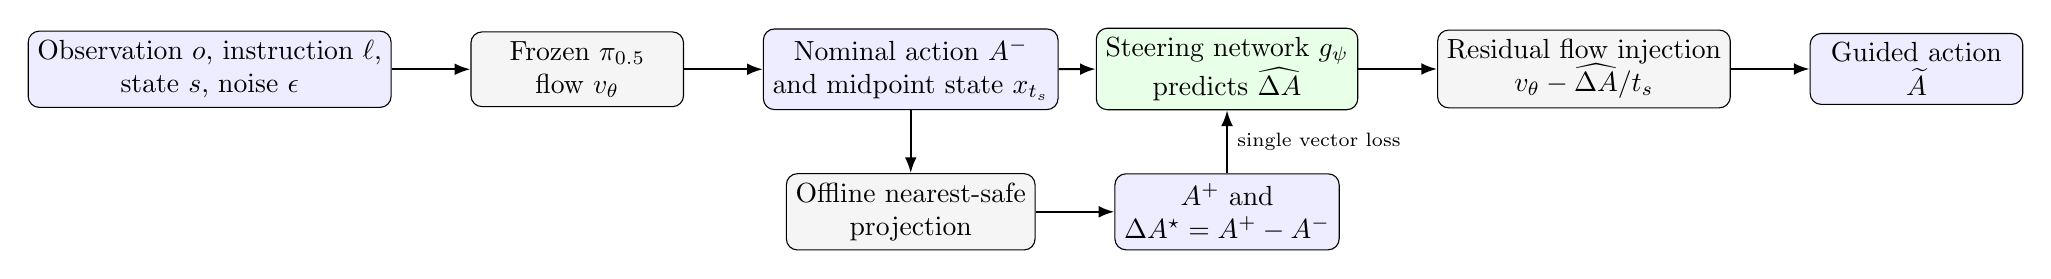
\begin{tikzpicture}[
    node distance=8mm and 10mm,
    box/.style={draw, rounded corners, align=center, minimum height=9mm, minimum width=27mm, fill=gray!8},
    data/.style={draw, rounded corners, align=center, minimum height=9mm, minimum width=27mm, fill=blue!7},
    learn/.style={draw, rounded corners, align=center, minimum height=9mm, minimum width=31mm, fill=green!9},
    arrow/.style={-{Latex[length=2mm]}, thick}
]
\node[data] (input) {Observation $o$, instruction $\ell$,\\state $s$, noise $\epsilon$};
\node[box, right=of input] (base) {Frozen \pizero{}\\flow $v_\theta$};
\node[data, right=of base] (nominal) {Nominal action $A^-$\\and midpoint state $x_{t_s}$};
\node[box, below=of nominal] (oracle) {Offline nearest-safe\\projection};
\node[data, right=of oracle] (target) {$A^+$ and\\$\Delta A^\star=A^+-A^-$};
\node[learn, above=of target] (steer) {Steering network $g_\psi$\\predicts $\widehat{\Delta A}$};
\node[box, right=of steer] (inject) {Residual flow injection\\$v_\theta-\widehat{\Delta A}/t_s$};
\node[data, right=of inject] (guided) {Guided action\\$\widetilde A$};

\draw[arrow] (input) -- (base);
\draw[arrow] (base) -- (nominal);
\draw[arrow] (nominal) -- (oracle);
\draw[arrow] (oracle) -- (target);
\draw[arrow] (nominal) -- (steer);
\draw[arrow] (target) -- node[right, font=\scriptsize] {single vector loss} (steer);
\draw[arrow] (steer) -- (inject);
\draw[arrow] (inject) -- (guided);
\end{tikzpicture}%
}
\caption{Overview of \method{}. Constrained optimization is used only offline to construct the minimal safe counterfactual. Deployment predicts a correction from an intermediate flow state and injects it as a residual velocity; no QP or CBF solver is used online.}
\label{fig:overview}
\end{figure*}

\subsection{Minimal safe counterfactual}

For each nominal prefix $A^-$, define the counterfactual action
\begin{equation}
\begin{aligned}
A^+ = \argmin_{A\in\mathcal{A}}
&\quad \frac{1}{2}\norm{A-A^-}_F^2\\
\text{s.t.}
&\quad D(A;s,G)\geq 0,\\
&\quad E(A;s)=E(A^-;s).
\end{aligned}
\label{eq:projection}
\end{equation}
Here $\mathcal{A}$ is the valid normalized action range. Equation~\eqref{eq:projection} is an offline label generator, not the learned objective and not an inference-time controller. It contains one optimization criterion: minimum action change. Safety and task preservation are hard constraints rather than weighted penalties.

If Eq.~\eqref{eq:projection} is infeasible, the example is marked infeasible rather than softened with extra penalty terms. If $A^-$ is already safe, then $A^+=A^-$. The supervision vector is
\begin{equation}
    \Delta A^\star=A^+-A^-.
    \label{eq:deltastar}
\end{equation}
Thus safe examples have exactly zero target correction.

\subsection{Endpoint-preserving correction subspace}

Under Eq.~\eqref{eq:kinematics}, endpoint change is linear in the action correction. Let $\delta a=\operatorname{vec}(\Delta A)\in\R^{3H}$ and
\begin{equation}
    B=\kappa[\,I_3\;I_3\;\cdots\;I_3\,]\in\R^{3\times 3H}.
\end{equation}
Endpoint preservation requires $B\delta a=0$. A network may output an unconstrained vector $z$, which is projected into the endpoint-preserving null space:
\begin{equation}
    \widehat{\delta a}
    =\Pi_{\mathrm{ep}}z,
    \qquad
    \Pi_{\mathrm{ep}}
    =I-B^\top(BB^\top)^{-1}B.
    \label{eq:nullspace}
\end{equation}
For the uniform translational model, Eq.~\eqref{eq:nullspace} is equivalent to subtracting the mean correction across the $H$ actions. This removes the need for an endpoint penalty in the training loss.

\subsection{Intermediate representation and steering model}

The base sampler is run normally from $t=1$ to a fixed intervention time $t_s$. The first experiment uses $t_s=0.5$, corresponding to the midpoint of the ten-step sampler. At that point we retain
\begin{equation}
    x_{t_s},
    \qquad
    \widehat A_{t_s}=x_{t_s}-t_s v_\theta(x_{t_s},t_s\mid o,\ell,s),
    \label{eq:predclean}
\end{equation}
where $\widehat A_{t_s}$ is the current predicted-clean action estimate implied by the training bridge in Eq.~\eqref{eq:flowbridge}.

The steering network receives
\begin{equation}
    \xi_{t_s}=\big[x_{t_s},\widehat A_{t_s},\phi(s,G),t_s\big]
\end{equation}
and predicts a raw correction $z=g_\psi(\xi_{t_s})$. The geometry encoding $\phi(s,G)$ is deliberately simple in the first study: obstacle pose and size in the current end-effector frame. The endpoint-preserving output is
\begin{equation}
    \widehat{\Delta A}=\operatorname{unvec}(\Pi_{\mathrm{ep}}z).
    \label{eq:predcorr}
\end{equation}
A small multilayer perceptron is sufficient for the first controlled experiment. Attention maps, image features, and action-expert hidden states are deferred until the basic mechanism is validated.

\subsection{Residual flow injection}

After predicting $\widehat{\Delta A}$ once at $t_s$, the remaining flow is integrated with
\begin{equation}
    \frac{dx_t}{dt}
    =v_\theta(x_t,t\mid o,\ell,s)
    -\frac{1}{t_s}\widehat{\Delta A},
    \qquad t\in[t_s,0].
    \label{eq:guidedflow}
\end{equation}
The correction is padded with zeros for non-translational dimensions and for actions beyond the executed prefix. Ignoring the change in the nonlinear base velocity caused by the edited state, the cumulative residual is
\begin{equation}
    \int_{t_s}^{0}-\frac{1}{t_s}\widehat{\Delta A}\,dt
    =\widehat{\Delta A}.
    \label{eq:integral}
\end{equation}
Hence the residual has a direct interpretation: it attempts to shift the final action by the predicted safe displacement. The equality is only exact for the additive residual term; the frozen base field is reevaluated at the modified states. Whether the nonlinear sampler retains the desired correction is therefore an empirical question tested by the oracle-steering experiment before any learned model is trusted.

With Euler step $\Delta t<0$, the update is
\begin{equation}
    x_{k+1}=x_k+\Delta t\left[
    v_\theta(x_k,t_k\mid o,\ell,s)
    -\frac{1}{t_s}\widehat{\Delta A}
    \right].
    \label{eq:euler}
\end{equation}

\subsection{Single training objective}

The frozen VLA is not updated. The only learned objective is
\begin{equation}
    \boxed{
    \mathcal{L}_{\mathrm{CRFS}}(\psi)
    =\E\left[
    \norm{\widehat{\Delta A}-\Delta A^\star}_F^2
    \right].}
    \label{eq:loss}
\end{equation}
No collision classifier, reward scalar, smoothness term, endpoint term, or task-success auxiliary head is used in the first study. Safe nominal examples contribute zero-vector targets.

\begin{algorithm}[t]
\caption{Offline counterfactual dataset construction}
\label{alg:data}
\begin{algorithmic}[1]
\Require Frozen VLA $v_\theta$, simulator state $S$, observation $o$, instruction $\ell$, obstacle $G$, noise $\epsilon$
\State Run the base sampler; save $x_{t_s}$ and nominal prefix $A^-$
\State Execute $A^-$ from $S$ and measure $D(A^-;S,G)$
\If{$D(A^-;S,G)\geq 0$}
    \State Set $A^+\gets A^-$
\Else
    \State Solve Eq.~\eqref{eq:projection} for $A^+$
    \If{infeasible} \State record infeasible case and stop \EndIf
    \State Verify $A^+$ in the simulator from the identical state $S$
\EndIf
\State Store $(x_{t_s},\widehat A_{t_s},\phi(S,G),\Delta A^\star)$
\end{algorithmic}
\end{algorithm}

\begin{algorithm}[t]
\caption{Learned steering at inference}
\label{alg:inference}
\begin{algorithmic}[1]
\Require Observation $o$, instruction $\ell$, state $s$, obstacle geometry $G$, noise $\epsilon$
\State Run frozen sampler from $t=1$ to $t=t_s$
\State Compute $\widehat A_{t_s}$ using Eq.~\eqref{eq:predclean}
\State Predict $z\gets g_\psi(x_{t_s},\widehat A_{t_s},\phi(s,G),t_s)$
\State Project $z$ with Eq.~\eqref{eq:nullspace} to obtain $\widehat{\Delta A}$
\State Continue sampling with Eq.~\eqref{eq:euler} until $t=0$
\State Return guided action chunk $\widetilde A$
\end{algorithmic}
\end{algorithm}

\section{Experimental Verification Plan}

The experiments are intentionally staged. A later stage is attempted only if the previous gate passes. This prevents model complexity from hiding a failure in geometry, feasibility, or the intervention point.

\subsection{Controlled pilot configuration}

The first experiment uses:
\begin{itemize}[leftmargin=*,nosep]
    \item one SafeLIBERO Level-II scenario with an obstacle directly in the movement path;
    \item one static, asymmetric, convex obstacle with simulator-known geometry;
    \item translational actions only;
    \item the first $H=5$ executed actions;
    \item the default ten-step OpenPI flow sampler and $t_s=0.5$;
    \item the same simulator state, observation, instruction, and noise for paired comparisons;
    \item episode-level train/validation/test splits, never random frame splits.
\end{itemize}

The asymmetry is important. A symmetric obstacle may admit equally short left and right detours, making the correction target multimodal. The first study should not mix a multimodal prediction problem with the more basic question of whether flow steering works at all.

A practical pilot collection target is at least 500 colliding and 500 already-safe nominal prefixes, generated across multiple episode initializations and noise samples. Counts may be increased after measuring the collision prevalence, but all thresholds and splits should be fixed before training the steering model.

\subsection{Ground-truth safety measurement}

The mechanism study uses the minimum signed geometry distance over every physics substep in MuJoCo \cite{todorov2012mujoco} of the five-action execution. A contact event is cross-checked against simulator contact pairs. This is more informative than the obstacle-displacement flag used in the released benchmark runner, which marks a collision after the obstacle position changes by more than a fixed threshold \cite{vlsarepo}. The original benchmark metric should still be reported later for comparability, but it should not be the supervision source for the proposed method.

Before collecting data, the following instrumentation tests are mandatory:
\begin{enumerate}[leftmargin=*,nosep]
    \item Restore the same simulator state and execute the same action prefix at least five times.
    \item Confirm that the measured minimum signed distance varies by less than $10^{-4}$ m.
    \item Confirm that reported first contact occurs near zero signed distance within the simulator's numerical tolerance.
    \item Visualize the geometry pair achieving the minimum distance and verify that it belongs to the end effector and designated obstacle.
\end{enumerate}

\subsection{Stage 0: measurement validity}

\paragraph{Question.} Is the continuous safety measurement reproducible and physically correct?

\paragraph{Pass condition.} All four instrumentation tests above pass on at least 50 diverse saved states.

\paragraph{Stop/refine condition.} If reproducibility or contact consistency fails, no learning experiment is run. The state-reset mechanism, geometry IDs, or substep tracker must be corrected first.

\subsection{Stage 1: counterfactual feasibility}

\paragraph{Question.} Does a local endpoint-preserving safe correction exist within the five-action horizon?

For every colliding nominal prefix, solve Eq.~\eqref{eq:projection}. Report
\begin{equation}
    F_{\mathrm{proj}}
    =P(A^+\text{ is feasible}\mid D(A^-)<0),
    \label{eq:fproj}
\end{equation}
\begin{equation}
    S_{\mathrm{teacher}}
    =P(D(A^+)\geq 0\mid A^+\text{ feasible}),
    \label{eq:teachersafe}
\end{equation}
and the median endpoint error after simulator execution,
\begin{equation}
    E_{\mathrm{teacher}}
    =\operatorname{median}\norm{E(A^+)-E(A^-)}_2.
    \label{eq:teacherend}
\end{equation}

\paragraph{Pilot pass condition.}
\begin{equation}
    F_{\mathrm{proj}}\geq 0.60,
    \qquad
    S_{\mathrm{teacher}}\geq 0.95,
    \qquad
    E_{\mathrm{teacher}}\leq 5\text{ mm}.
\end{equation}
These are pre-registered pilot gates, not universal safety standards.

\paragraph{Stop/refine condition.}
If $S_{\mathrm{teacher}}<0.95$, the label construction is not trustworthy and the solver or geometry model must be fixed. If $F_{\mathrm{proj}}<0.40$, repeat only once with $H=10$. If feasibility remains below $0.60$, the local endpoint-preserving premise is considered false for this task; the project should pivot to longer-horizon planning or earlier intervention rather than adding a more complex network.

\subsection{Stage 2: oracle flow steerability}

\paragraph{Question.} If the exact correction $\Delta A^\star$ is known, can the residual flow in Eq.~\eqref{eq:guidedflow} turn the same observation--noise sample into a safe action?

For each feasible colliding example, compare:
\begin{enumerate}[leftmargin=*,nosep]
    \item \textbf{Base:} no intervention;
    \item \textbf{Random residual:} an endpoint-preserving random vector with the same norm as $\Delta A^\star$;
    \item \textbf{Oracle residual:} the exact $\Delta A^\star$;
    \item \textbf{Direct oracle action:} execute $A^+$ directly, serving only as an upper bound.
\end{enumerate}
All conditions use the same saved state and the same initial flow noise.

Let $\widetilde A_{\mathrm{oracle}}$ and $\widetilde A_{\mathrm{rand}}$ denote the final sampled actions. The primary quantities are
\begin{equation}
R_{\mathrm{oracle}}
=P\big(D(\widetilde A_{\mathrm{oracle}})\geq 0
\mid D(A^-)<0, A^+\text{ feasible}\big),
\label{eq:roracle}
\end{equation}
\begin{equation}
R_{\mathrm{rand}}
=P\big(D(\widetilde A_{\mathrm{rand}})\geq 0
\mid D(A^-)<0, A^+\text{ feasible}\big),
\label{eq:rrand}
\end{equation}
and the median local endpoint error of the oracle-guided action.

\paragraph{Pilot pass condition.}
The oracle intervention is considered meaningfully steerable when
\begin{equation}
    R_{\mathrm{oracle}}\geq 0.50,
    \qquad
    R_{\mathrm{oracle}}-R_{\mathrm{rand}}\geq 0.20,
\end{equation}
with a paired 95\% bootstrap confidence interval for the difference strictly above zero, and with median endpoint error below 1 cm.

\paragraph{Stop/refine condition.}
If the midpoint intervention fails, test only two later intervention times, $t_s\in\{0.3,0.1\}$. If no intervention time significantly exceeds the equal-norm random residual, action-flow steering is rejected for this formulation. The next research direction should change the intervention representation or directly adapt the action expert, rather than train a predictor for a non-causal direction.

\subsection{Stage 3: learned correction}

\paragraph{Question.} Can the correction be predicted from the intermediate flow state and simple obstacle geometry?

Train $g_\psi$ with Eq.~\eqref{eq:loss}. The test set must contain held-out episode initializations and obstacle poses. The mandatory comparisons are:
\begin{enumerate}[leftmargin=*,nosep]
    \item base \pizero{};
    \item equal-norm random residual;
    \item best-of-$8$ noise seeds, to test whether sampling alone can find safe support;
    \item learned \method{};
    \item oracle residual, as the achievable upper bound for this intervention mechanism.
\end{enumerate}

For colliding nominal samples, define the learned rescue rate
\begin{equation}
R_{\mathrm{learned}}
=P\big(D(\widetilde A_{\mathrm{learned}})\geq 0\mid D(A^-)<0\big).
\label{eq:rlearned}
\end{equation}
For already-safe nominal samples, define safe preservation
\begin{equation}
P_{\mathrm{preserve}}
=P\big(D(\widetilde A_{\mathrm{learned}})\geq 0\mid D(A^-)\geq 0\big).
\label{eq:preserve}
\end{equation}
The fraction of the oracle steering gap recovered is
\begin{equation}
\rho
=\frac{R_{\mathrm{learned}}-R_{\mathrm{rand}}}
{R_{\mathrm{oracle}}-R_{\mathrm{rand}}}.
\label{eq:rho}
\end{equation}

\paragraph{Pilot pass condition.}
Proceed to closed-loop evaluation when
\begin{equation}
    \rho\geq 0.50,
    \qquad
    P_{\mathrm{preserve}}\geq 0.95,
\end{equation}
and the learned intervention maintains median endpoint error below 1 cm. Learned rescue must also significantly exceed best-of-$8$ seed selection on the subset where all eight base samples are unsafe.

\paragraph{Stop/refine condition.}
If training error is low but test rescue is poor, the issue is generalization; add obstacle-pose and state diversity before changing the loss. If training error itself is high, inspect target multimodality and input sufficiency. Permit only two refinements before reassessing the premise: doubling the dataset and one architecture/input revision. If $\rho<0.30$ after both, the correction is not sufficiently predictable from the chosen intermediate representation and the idea should pivot to a richer representation or direct residual-flow fine-tuning.

\subsection{Stage 4: closed-loop utility}

\paragraph{Question.} Does the learned intervention improve complete task execution rather than only five-action clips?

Run full episodes with:
\begin{enumerate}[leftmargin=*,nosep]
    \item base \pizero{};
    \item best-of-$8$ seed selection;
    \item learned \method{};
    \item AEGIS as an external analytic safety reference;
    \item optionally, \method{} followed by AEGIS, to test complementarity rather than replacement.
\end{enumerate}

The primary episode metric is
\begin{equation}
\begin{aligned}
\mathrm{SafeSuccess}=P(&\text{task succeeds}\;\land\;\\
&\text{no forbidden collision occurs}).
\end{aligned}
\label{eq:safesuccess}
\end{equation}
Collision avoidance rate and ordinary task success rate are reported separately because a policy can appear safe by stopping, and can complete a task despite an unsafe collision. The VLSA benchmark likewise reports collision avoidance and task success separately \cite{hu2025vlsa}.

\paragraph{Pilot pass condition.}
The direction is considered worthy of broader study when learned \method{} improves SafeSuccess by at least five percentage points over the base policy with a paired 95\% confidence interval above zero, while ordinary task success decreases by no more than five percentage points. The adapter should also add less than 10\% to VLA inference latency.

\paragraph{Stop/refine condition.}
If clip-level rescue succeeds but closed-loop SafeSuccess does not improve, inspect whether corrections drive the policy into out-of-distribution states, a failure mode also discussed for safety interventions in VLSA \cite{hu2025vlsa}. One data-aggregation round is allowed: collect states reached by the guided policy, rebuild counterfactual labels there, and retrain. If SafeSuccess still does not improve, the method is not worthwhile in its current local form.

\section{Decision Table}

\begin{table*}[t]
\centering
\caption{Pre-registered decision gates. Thresholds are pilot criteria chosen to prevent indefinite iteration; they are not claims of deployment-level safety.}
\label{tab:gates}
\setlength{\tabcolsep}{5pt}
\begin{tabular}{p{1.35cm}p{3.6cm}p{4.8cm}p{5.0cm}}
\toprule
Stage & Core question & Continue criterion & Stop or refine action \\
\midrule
0 & Is the signed-distance measurement valid? & Repeatability $<10^{-4}$ m and contact-consistent geometry on 50 states & Stop all model work; repair state restoration, geom IDs, or substep measurement \\
1 & Does a local safe equivalent exist? & $F_{\mathrm{proj}}\geq0.60$, teacher safety $\geq0.95$, endpoint error $\leq5$ mm & If low feasibility, try $H=10$ once; if still low, pivot to longer-horizon planning \\
2 & Is the flow causally steerable? & $R_{\mathrm{oracle}}\geq0.50$, at least 20-point gain over random, endpoint error $\leq1$ cm & Try $t_s=0.3$ and $0.1$ only; if all fail, reject this action-flow intervention \\
3 & Is the direction learnable? & $\rho\geq0.50$, safe preservation $\geq0.95$, and beats best-of-$8$ on all-unsafe groups & Double data and change input/architecture once; if $\rho<0.30$, pivot representation or training method \\
4 & Is it useful closed loop? & SafeSuccess $+5$ points or more, confidence interval above zero, task-success loss $\leq5$ points & One guided-state data-aggregation round; if still no gain, stop the local method \\
\bottomrule
\end{tabular}
\end{table*}

\section{Statistical Protocol}

All mechanism comparisons are paired by simulator state and flow noise. Confidence intervals are obtained by bootstrapping complete episodes or state groups, not individual frames. Seeds from the same state must remain in the same train, validation, or test split. Report absolute rates, paired differences, and 95\% confidence intervals. Hyperparameters, intervention times, and pass criteria are fixed before observing test results.

The strongest evidence against the seed-selection explanation is the \emph{all-sampled-unsafe} subset. For each state, draw eight base noise samples. Retain groups for which all eight nominal prefixes collide. A successful learned residual on these groups demonstrates that the method is not merely selecting an already-safe base sample.

\section{Implementation Plan in the Released Codebase}

The implementation requires three localized changes:
\begin{enumerate}[leftmargin=*,nosep]
    \item \textbf{Expose the intervention state.} Modify the OpenPI PyTorch sampler to return $x_{t_s}$ and the velocity at the chosen Euler step. The current implementation initializes $x_t$ with Gaussian noise, uses ten Euler steps by default, and returns only the final action chunk \cite{openpirepo,vlsarepo}.
    \item \textbf{Add residual integration.} After $t_s$, subtract $\widehat{\Delta A}/t_s$ from the translational prefix of the predicted velocity at each remaining Euler step.
    \item \textbf{Branch and measure.} From a saved simulator state, execute nominal, random, oracle, and learned actions separately. Track minimum end-effector--obstacle signed distance at every physics substep. The released runner already exposes a five-step replanning parameter and a safe-success log, but its displacement-based collision flag should not be used as the continuous supervision target \cite{vlsarepo}.
\end{enumerate}

No change to the pretrained VLA weights is required in the first version. The steering network can be trained independently from stored intermediate states and counterfactual vectors.

\section{What Is Deliberately Deferred}

The following additions are scientifically reasonable but should be attempted only after the five gates in Table~\ref{tab:gates}:
\begin{itemize}[leftmargin=*,nosep]
    \item full rotational actions and gripper corrections;
    \item action-expert hidden states or attention maps as steering inputs;
    \item multiple obstacles and full-arm collision geometry;
    \item learned visual obstacle perception instead of simulator-known geometry;
    \item multimodal corrections around symmetric obstacles;
    \item repeated feedback prediction of $\widehat{\Delta A}$ at every flow step;
    \item real-robot deployment.
\end{itemize}

This ordering is important. A negative result at an earlier gate provides actionable information. Adding more labels, auxiliary losses, or perception modules before establishing oracle steerability would make the source of failure ambiguous.

\section{Limitations and Non-Claims}

\method{} has no formal forward-invariance guarantee. The offline projection may be infeasible, the learned correction may generalize poorly, and endpoint preservation is only a local proxy for task intent. The controlled first study covers end-effector translation around one static obstacle and does not address arm-link collisions, dynamic agents, grasp contact semantics, or global planning. The method may also induce distribution shift by moving the robot into states rarely visited by the base policy. These limitations are not hidden by the experimental design; they are exactly what the stage-wise gates are intended to expose.

\section{Expected Research Outcome}

A successful result would support the following limited claim:

\begin{quote}
For a controlled collision-avoidance setting, an intermediate action-flow state of a frozen \pizero{} policy admits an endpoint-preserving safety displacement, and a compact learned residual can recover a substantial fraction of the oracle steering effect without online constrained optimization.
\end{quote}

A failure is also informative. Low projection feasibility rejects the local-detour assumption; failed oracle steering rejects the chosen flow intervention; failed learning identifies a representation or multimodality bottleneck; failed closed-loop utility exposes safety-induced distribution shift. The proposal is therefore designed to determine quickly whether the idea deserves expansion rather than to accumulate engineering complexity around an unverified premise.

\bibliographystyle{IEEEtran}
\bibliography{references}

\end{document}
